% 2002 年春季上海卷第 12 题：平面三角形与空间三棱锥比例
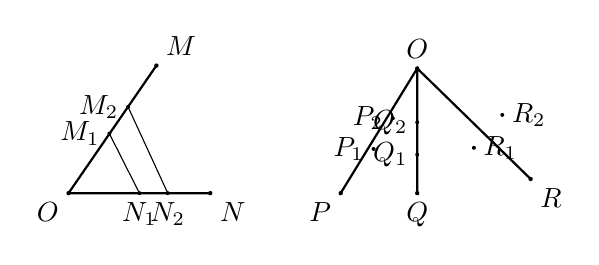
\begin{tikzpicture}[>=stealth, scale=0.72]
  % 两条共面射线
  \begin{scope}
    \coordinate (O) at (0,0);
    \coordinate (M) at (1.55,2.25);
    \coordinate (N) at (2.5,0);
    \coordinate (Mone) at (0.72,1.05);
    \coordinate (Mtwo) at (1.05,1.52);
    \coordinate (None) at (1.25,0);
    \coordinate (Ntwo) at (1.75,0);
    \draw[thick] (O)--(M) (O)--(N);
    \draw (Mone)--(None) (Mtwo)--(Ntwo);
    \fill (O) circle (1.1pt) node[below left] {$O$};
    \fill (M) circle (1.1pt) node[above right] {$M$};
    \fill (N) circle (1.1pt) node[below right] {$N$};
    \fill (Mone) circle (1.0pt) node[left] {$M_1$};
    \fill (Mtwo) circle (1.0pt) node[left] {$M_2$};
    \fill (None) circle (1.0pt) node[below] {$N_1$};
    \fill (Ntwo) circle (1.0pt) node[below] {$N_2$};
  \end{scope}

  % 三条不共面射线的透视示意
  \begin{scope}[xshift=4.8cm]
    \coordinate (Otwo) at (1.35,2.2);
    \coordinate (P) at (0,0);
    \coordinate (Q) at (1.35,0);
    \coordinate (R) at (3.35,0.25);
    \draw[thick] (Otwo)--(P) (Otwo)--(Q) (Otwo)--(R);
    \coordinate (Pone) at (0.58,0.78);
    \coordinate (Ptwo) at (0.92,1.32);
    \coordinate (Qone) at (1.35,0.68);
    \coordinate (Qtwo) at (1.35,1.25);
    \coordinate (Rone) at (2.35,0.80);
    \coordinate (Rtwo) at (2.85,1.38);
    \fill (Otwo) circle (1.1pt) node[above] {$O$};
    \fill (P) circle (1.1pt) node[below left] {$P$};
    \fill (Q) circle (1.1pt) node[below] {$Q$};
    \fill (R) circle (1.1pt) node[below right] {$R$};
    \fill (Pone) circle (1.0pt) node[left] {$P_1$};
    \fill (Ptwo) circle (1.0pt) node[left] {$P_2$};
    \fill (Qone) circle (1.0pt) node[left] {$Q_1$};
    \fill (Qtwo) circle (1.0pt) node[left] {$Q_2$};
    \fill (Rone) circle (1.0pt) node[right] {$R_1$};
    \fill (Rtwo) circle (1.0pt) node[right] {$R_2$};
  \end{scope}
\end{tikzpicture}
